\documentclass[a4paper]{report}

\usepackage{graphicx}
\usepackage{amsmath,amssymb}
\usepackage{float}
\usepackage{hyperref}

\title{BPropy report}

\begin{document}

\tableofcontents

\section{Definitions}

\subsection{Erdos-Renyi graph generator}
The Erdos-Renyi Graph $G(n,p)$ with $n$ nodes and edge probability $p$ is generated by including each edge with probability $p$ independently from every other edge.

\subsection{Target probability over pools of solution}
We are given a graph $G$ and a pool of solutions $\mathcal{P} = \{ y_i \}_{i\in\mathbb{N}}$. Each solution $y_i$ has cost $c(y_i)$ and the \emph{target weighted probability} over unary variable assignments are $$\overline{y}_i = \frac{1}{Z}\sum\limits_{y\in\mathcal{P}} \exp c(y) y_i$$ 
with $Z = \sum\limits_{y\in\mathcal{P}} \exp c(y)$. 



\section{Dataset details}


\begin{center}
\begin{tabular}{lccccccc}
\hline
	Id & $n$ & $p$ & $N_{\text{train}}$ & $N_{\text{test}}$ & RelGap & AbsGap & Weights\\
	\hline
	maxcut n100 p0.15         & $100$ & $0.15$ & $1000$ & $100$ & None & None & $w_i=1$\\
	maxcut n100 p0.15 uniform & $100$ & $0.15$ & $1000$ & $100$ & None & None & $w_i \sim \mathcal{U}[0,1]$ \\
	maxcut n100 p0.15 exp & $100$ & $0.15$ & $1000$ & $100$ & None & None & $w_i \sim \mathcal{E}[1]$ \\
	maxcut n100 p0.15 normal & $100$ & $0.15$ & $1000$ & $100$ & None & None & $w_i \sim \mathcal{N}[0,1]$


\end{tabular}
\end{center}

\begin{center}
\begin{tabular}{lccc}
\hline
	Id & Train loss & Val loss & Gap (\%) \\
	\hline
	maxcut n100 p0.15 uniform & 0.02 & 0.02 &  40 \\
	maxcut n100 p0.15 &0.00765 & 0.00644 & 27 \\
\end{tabular}
\end{center}



\subsection{Maxcut n100 p0.15}

\begin{figure}[H]
	\centering
	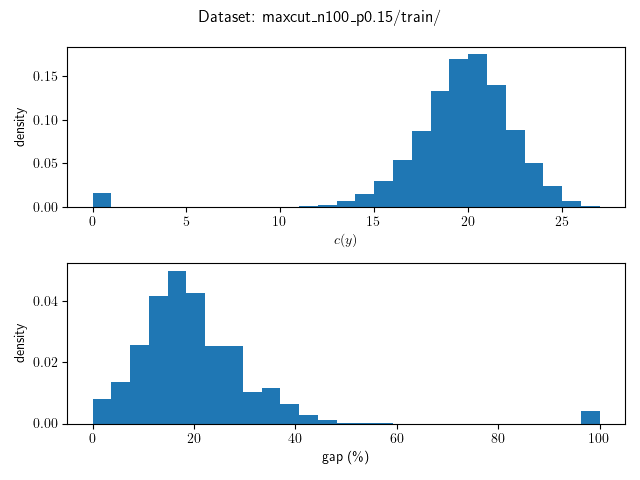
\includegraphics[width=.9\textwidth]{maxcut_n100_p0.15_hist_cost_gap.png}
	\caption{Top: distribution of the solution costs over the entire dataset. Bottom: distribution of the solution optimality gap over entire dataset}
\end{figure}

\begin{figure}[H]
	\centering
	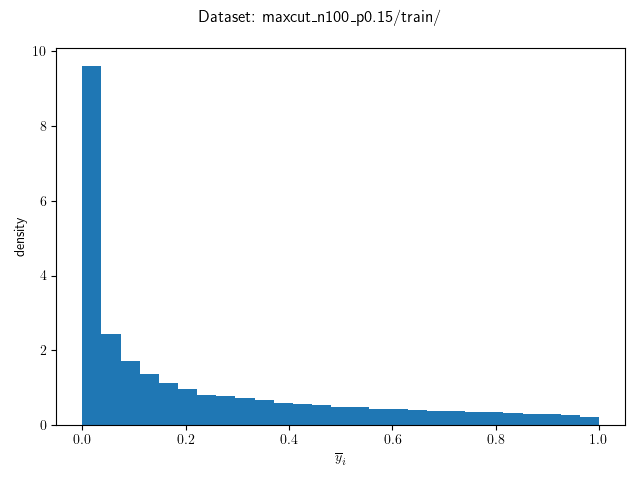
\includegraphics[width=.9\textwidth]{maxcut_n100_p0.15_hist_target.png}
	\caption{Distribution of target probabilities over entire dataset}
\end{figure}

\begin{figure}[H]
	\centering
	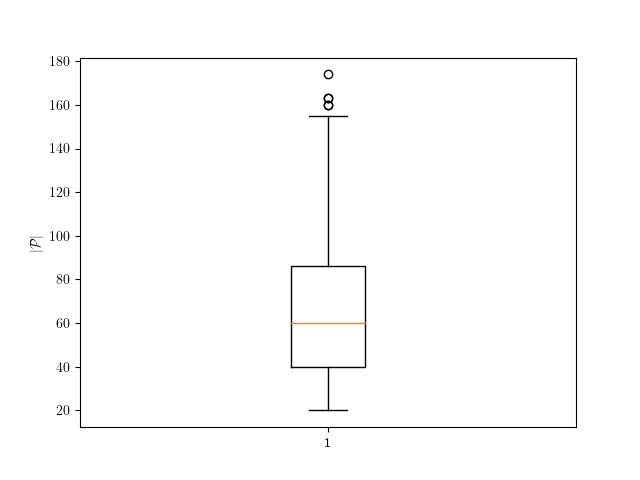
\includegraphics[width=.9\textwidth]{maxcut_n100_p0.15_boxplot_pool.png}
	\caption{Distribution of the number of solutions in each solution pool}
\end{figure}

\begin{figure}[H]
	\centering
	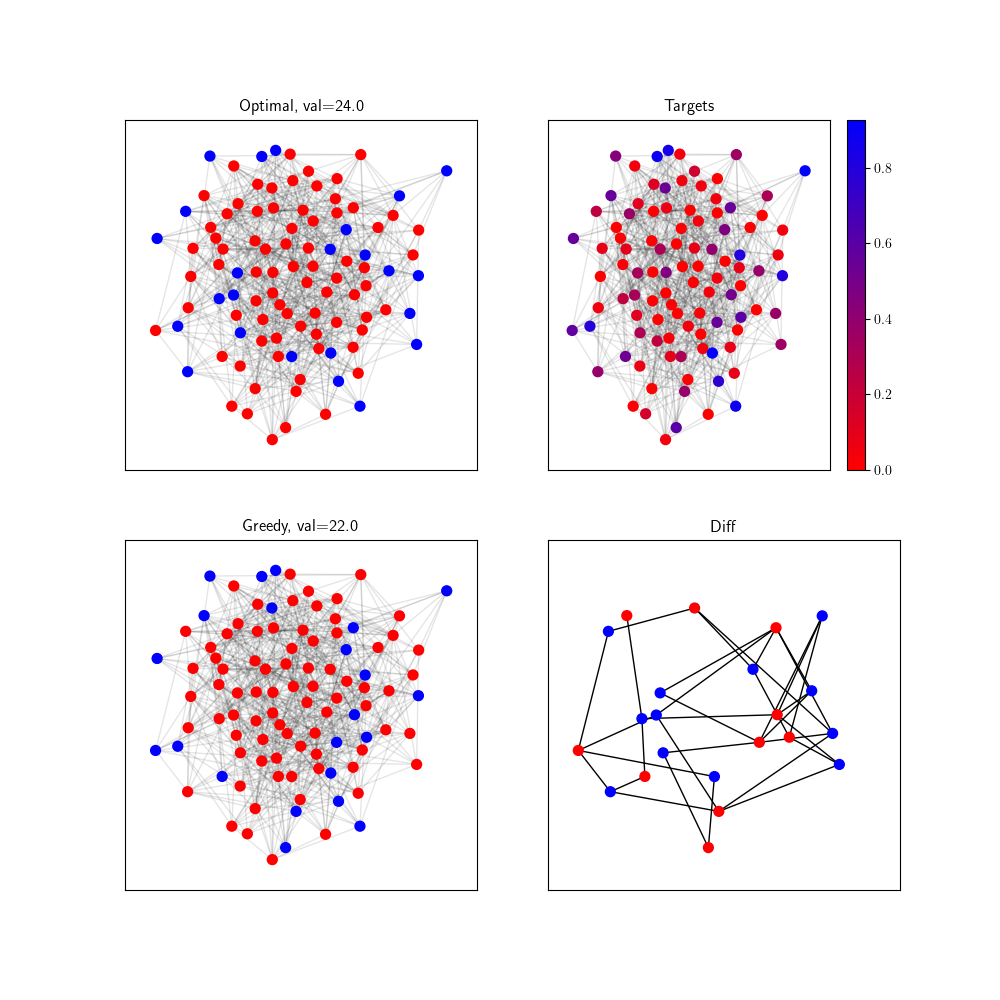
\includegraphics[width=.9\textwidth]{maxcut_n100_p0.15_graph_sol.png}
	\caption{Top left: original graph and optimal solution (blue nodes), Top Right: node colors function of $\overline{y}_i$ (red to blue), Bottom left: solution obtained with greedy procedure with costs $\{ \overline{y}_i \}$, Bottom right: subgraph defined by nodes belonging to either the optimal solution (blue) or the greedy solution (red)}
\end{figure}

\newpage
\subsection{Maxcut n100 p0.15 uniform}

\begin{figure}[H]
	\centering
	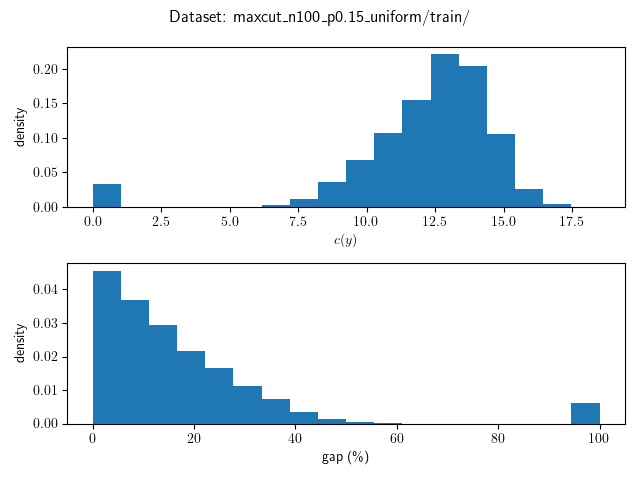
\includegraphics[width=.9\textwidth]{maxcut_n100_p0.15_uniform_hist_cost_gap.png}
	\caption{Top: distribution of the solution costs over the entire dataset. Bottom: distribution of the solution optimality gap over entire dataset}

\end{figure}

\begin{figure}[H]
	\centering
	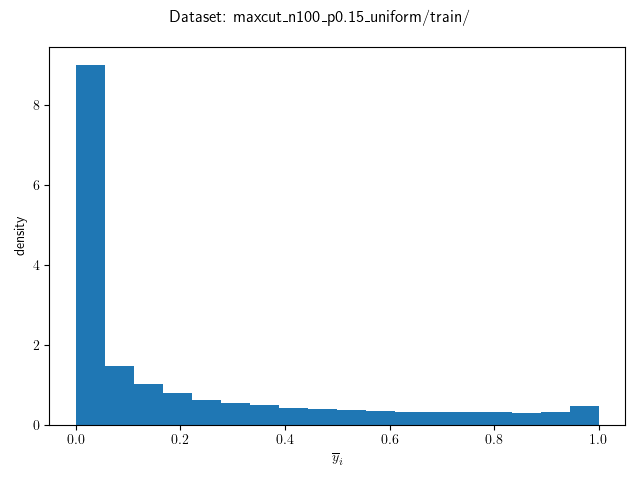
\includegraphics[width=.9\textwidth]{maxcut_n100_p0.15_uniform_hist_target.png}
	\caption{Distribution of target probabilities over entire dataset}

\end{figure}

\begin{figure}[H]
	\centering
	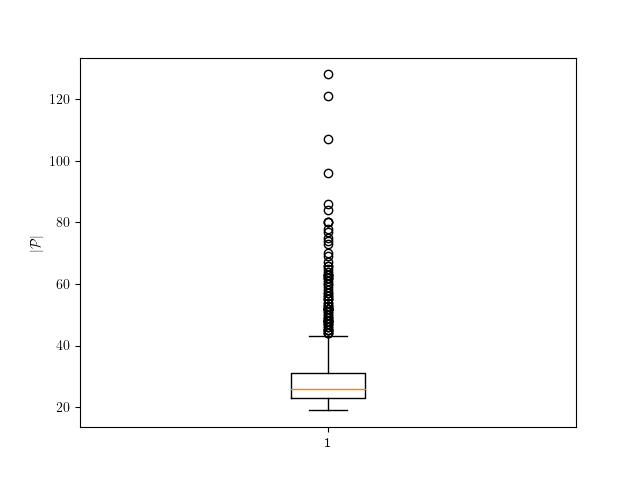
\includegraphics[width=.9\textwidth]{maxcut_n100_p0.15_uniform_boxplot_pool.png}
	\caption{Distribution of the number of solutions in each solution pool}

\end{figure}

\begin{figure}[H]
	\centering
	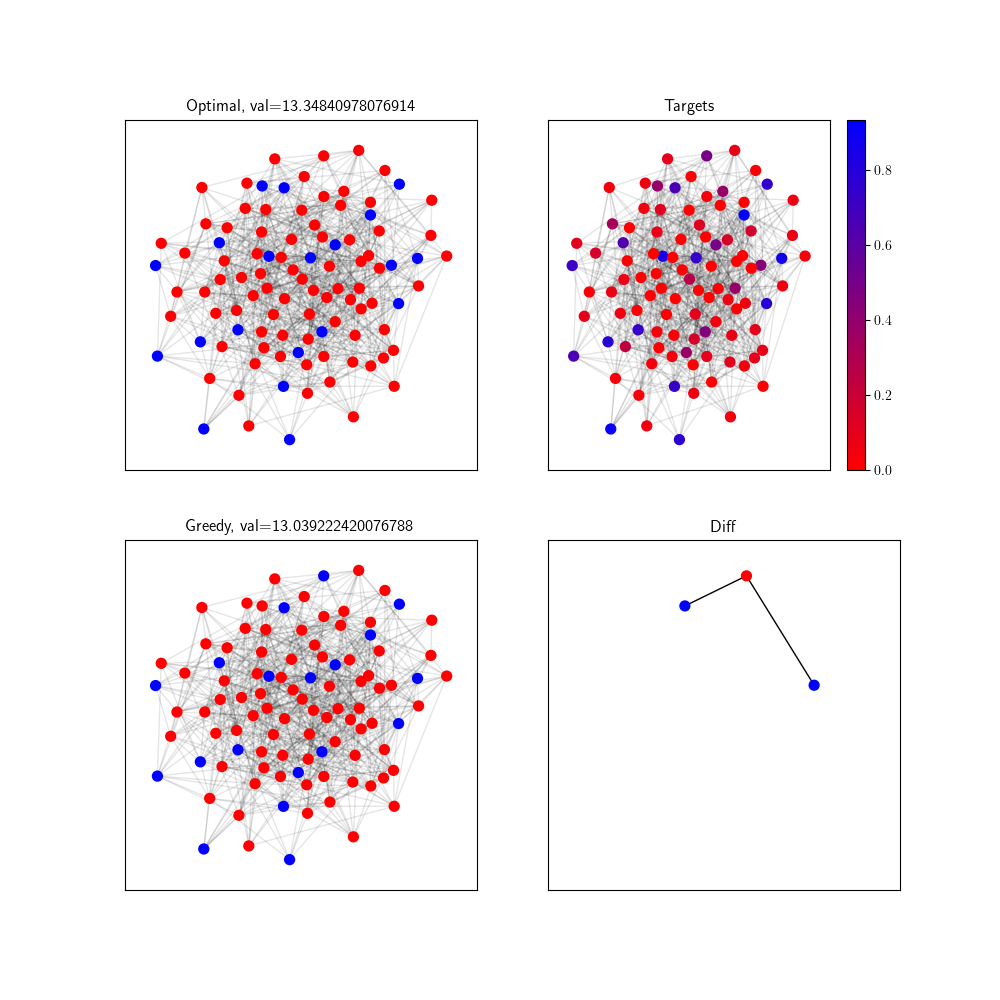
\includegraphics[width=.9\textwidth]{maxcut_n100_p0.15_uniform_graph_sol.png}
	\caption{Top left: original graph and optimal solution (blue nodes), Top Right: node colors function of $\overline{y}_i$ (red to blue), Bottom left: solution obtained with greedy procedure with costs $\{ \overline{y}_i \}$, Bottom right: subgraph defined by nodes belonging to either the optimal solution (blue) or the greedy solution (red)}

\end{figure}

\begin{figure}[H]
	\centering
	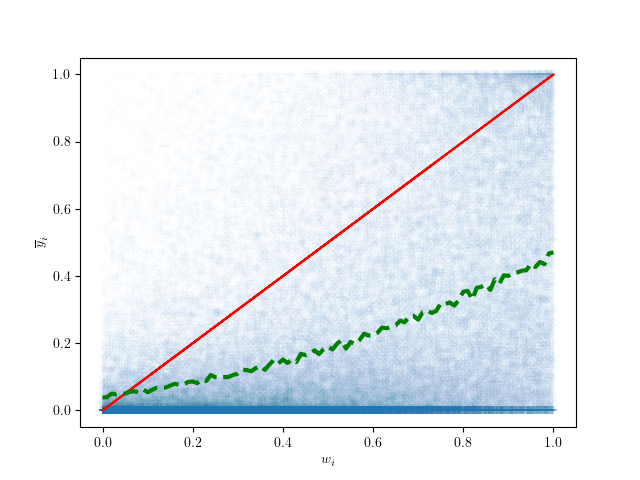
\includegraphics[width=.9\textwidth]{maxcut_n100_p0.15_uniform_scatter_weight_target.png}
	\caption{Scatter plot of target $\overline{y}_i$ as a function of the cost $w_i$ of node $i$. Green line is a rolling mean value}
\end{figure}

\begin{figure}[H]
	\centering
	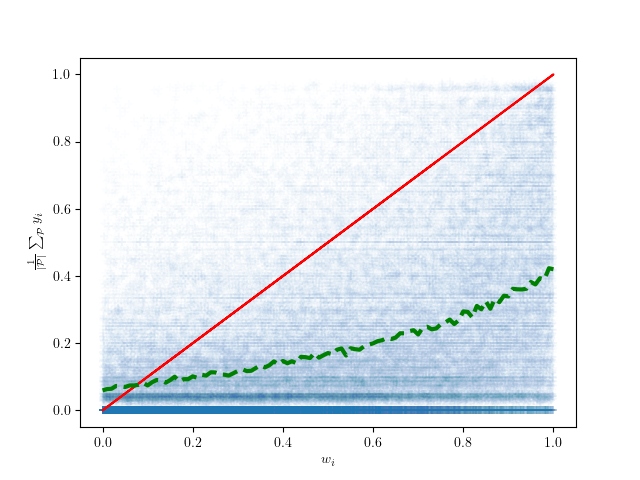
\includegraphics[width=.9\textwidth]{maxcut_n100_p0.15_uniform_scatter_weight_prop.png}
	\caption{Scatter plot of proportion $\frac{1}{|\mathcal{P}|} \sum_{\mathcal{P}} y_i$ as a function of the cost $w_i$ of node $i$. Green line is a rolling mean value}

\end{figure}

\newpage
\subsection{Maxcut n100 p0.15 exp}

\begin{figure}[H]
	\centering
	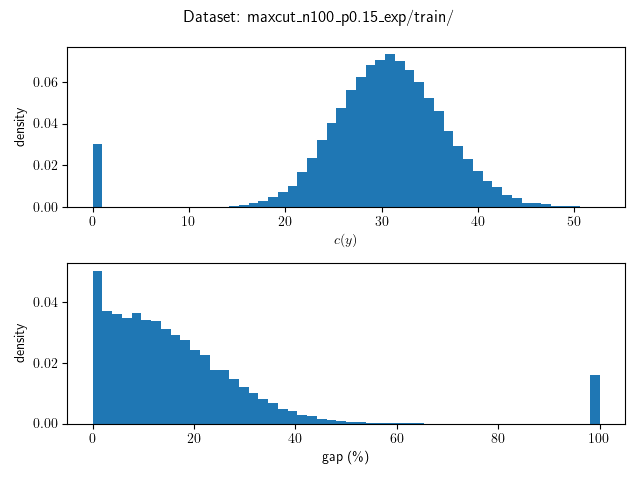
\includegraphics[width=.9\textwidth]{maxcut_n100_p0.15_exp_hist_cost_gap.png}
	\caption{Top: distribution of the solution costs over the entire dataset. Bottom: distribution of the solution optimality gap over entire dataset}

\end{figure}

\begin{figure}[H]
	\centering
	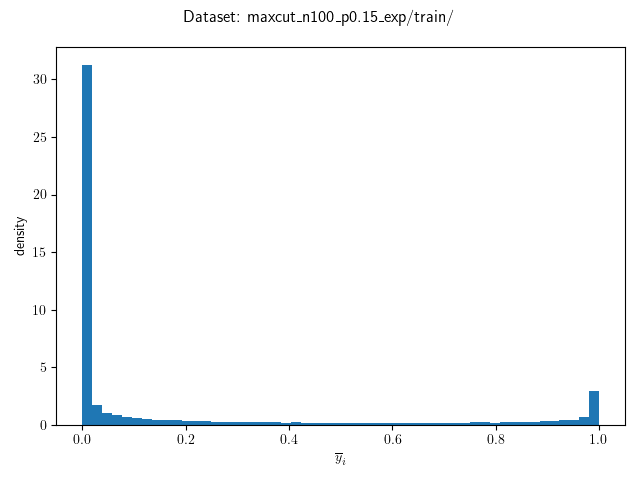
\includegraphics[width=.9\textwidth]{maxcut_n100_p0.15_exp_hist_target.png}
	\caption{Distribution of target probabilities over entire dataset}

\end{figure}

\begin{figure}[H]
	\centering
	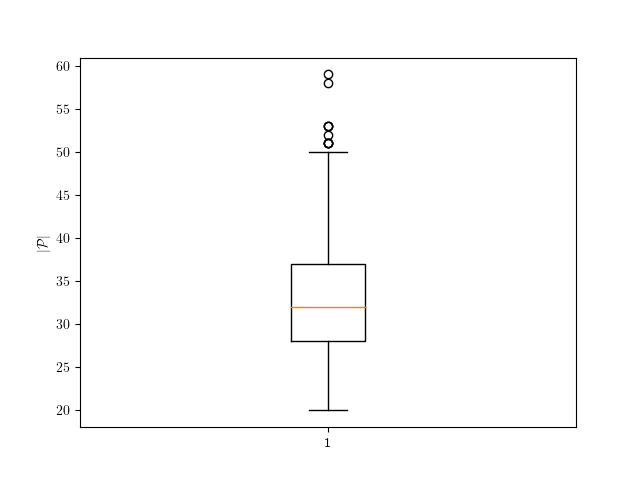
\includegraphics[width=.9\textwidth]{maxcut_n100_p0.15_exp_boxplot_pool.png}
	\caption{Distribution of the number of solutions in each solution pool}

\end{figure}

\begin{figure}[H]
	\centering
	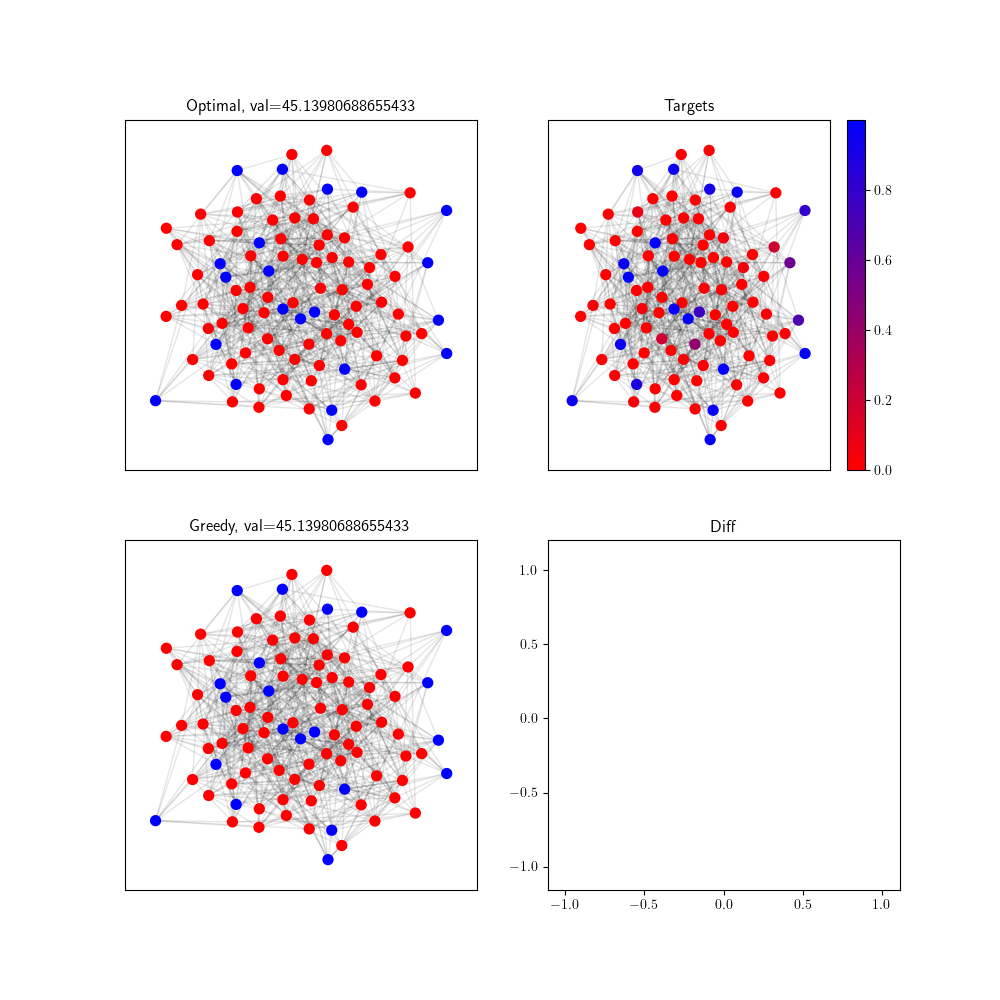
\includegraphics[width=.9\textwidth]{maxcut_n100_p0.15_exp_graph_sol.png}
	\caption{Top left: original graph and optimal solution (blue nodes), Top Right: node colors function of $\overline{y}_i$ (red to blue), Bottom left: solution obtained with greedy procedure with costs $\{ \overline{y}_i \}$, Bottom right: subgraph defined by nodes belonging to either the optimal solution (blue) or the greedy solution (red)}

\end{figure}

\begin{figure}[H]
	\centering
	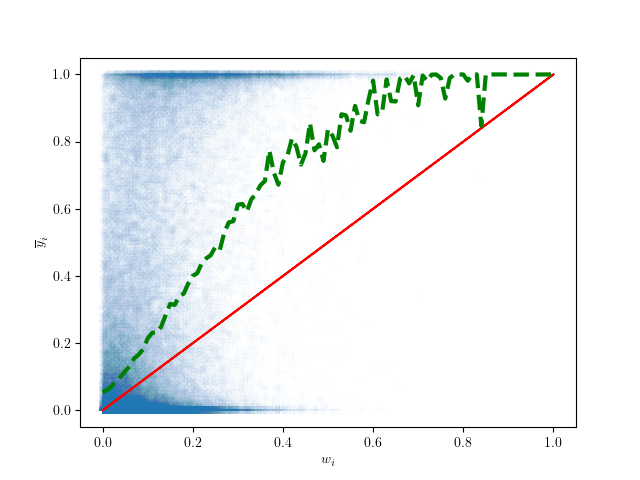
\includegraphics[width=.9\textwidth]{maxcut_n100_p0.15_exp_scatter_weight_target.png}
	\caption{Scatter plot of target $\overline{y}_i$ as a function of the cost $w_i$ of node $i$. Green line is a rolling mean value}
\end{figure}

\begin{figure}[H]
	\centering
	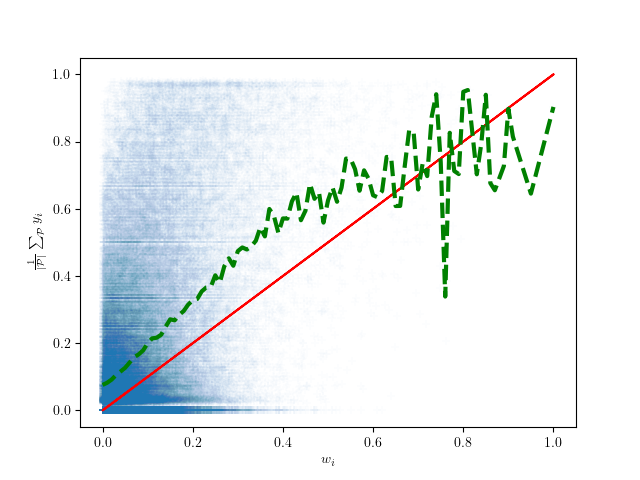
\includegraphics[width=.9\textwidth]{maxcut_n100_p0.15_exp_scatter_weight_prop.png}
	\caption{Scatter plot of proportion $\frac{1}{|\mathcal{P}|} \sum_{\mathcal{P}} y_i$ as a function of the cost $w_i$ of node $i$. Green line is a rolling mean value}

\end{figure}

\newpage
\subsection{Maxcut n100 p0.15 normal}

\begin{figure}[H]
	\centering
	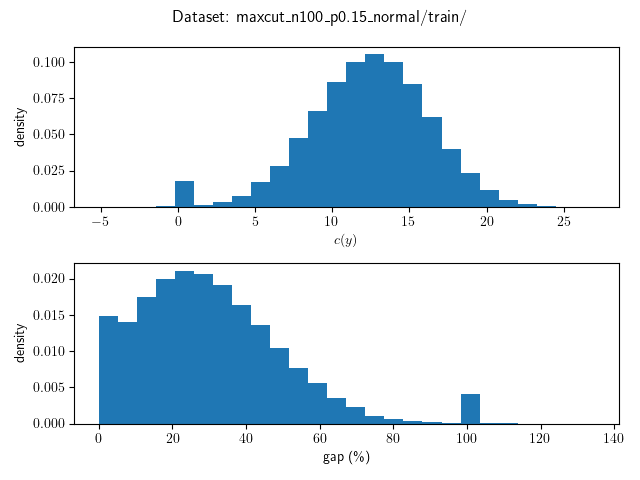
\includegraphics[width=.9\textwidth]{maxcut_n100_p0.15_normal_hist_cost_gap.png}
	\caption{Top: distribution of the solution costs over the entire dataset. Bottom: distribution of the solution optimality gap over entire dataset}

\end{figure}

\begin{figure}[H]
	\centering
	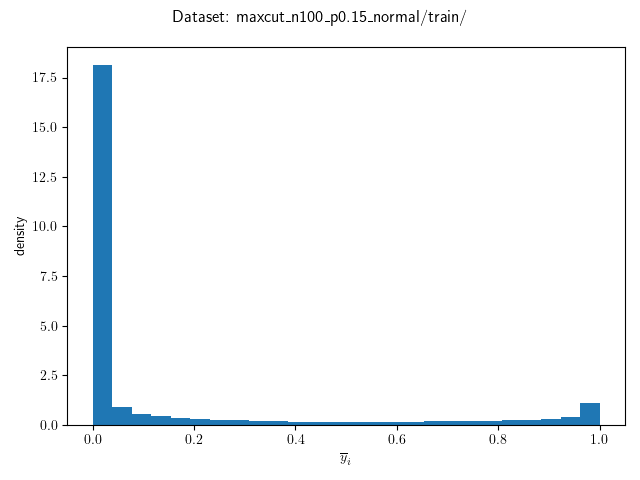
\includegraphics[width=.9\textwidth]{maxcut_n100_p0.15_normal_hist_target.png}
	\caption{Distribution of target probabilities over entire dataset}

\end{figure}

\begin{figure}[H]
	\centering
	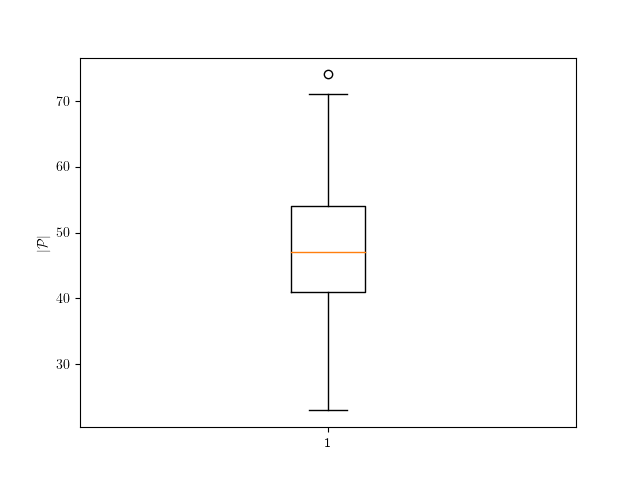
\includegraphics[width=.9\textwidth]{maxcut_n100_p0.15_normal_boxplot_pool.png}
	\caption{Distribution of the number of solutions in each solution pool}

\end{figure}

\begin{figure}[H]
	\centering
	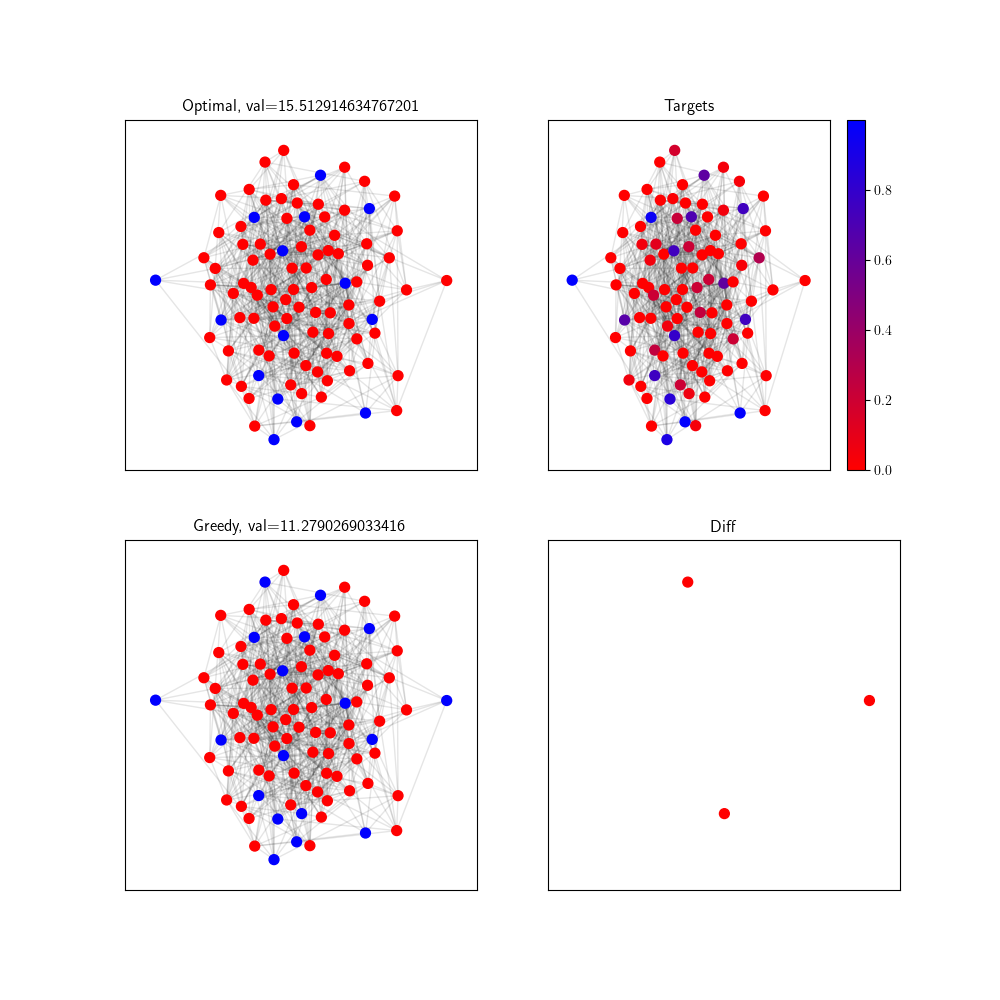
\includegraphics[width=.9\textwidth]{maxcut_n100_p0.15_normal_graph_sol.png}
	\caption{Top left: original graph and optimal solution (blue nodes), Top Right: node colors function of $\overline{y}_i$ (red to blue), Bottom left: solution obtained with greedy procedure with costs $\{ \overline{y}_i \}$, Bottom right: subgraph defined by nodes belonging to either the optimal solution (blue) or the greedy solution (red)}

\end{figure}

\begin{figure}[H]
	\centering
	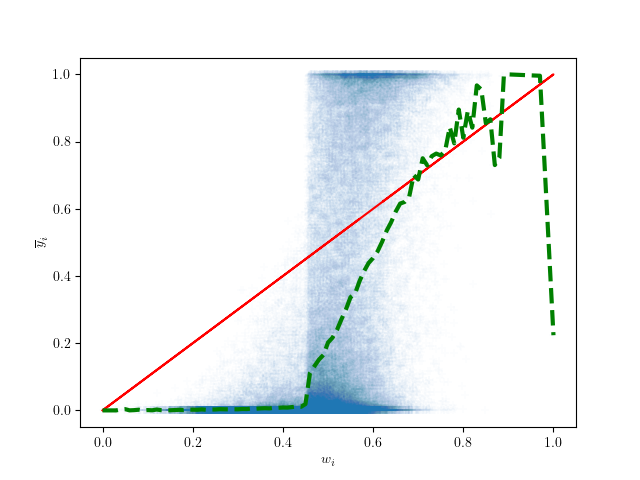
\includegraphics[width=.9\textwidth]{maxcut_n100_p0.15_normal_scatter_weight_target.png}
	\caption{Scatter plot of target $\overline{y}_i$ as a function of the cost $w_i$ of node $i$. Green line is a rolling mean value}
\end{figure}

\begin{figure}[H]
	\centering
	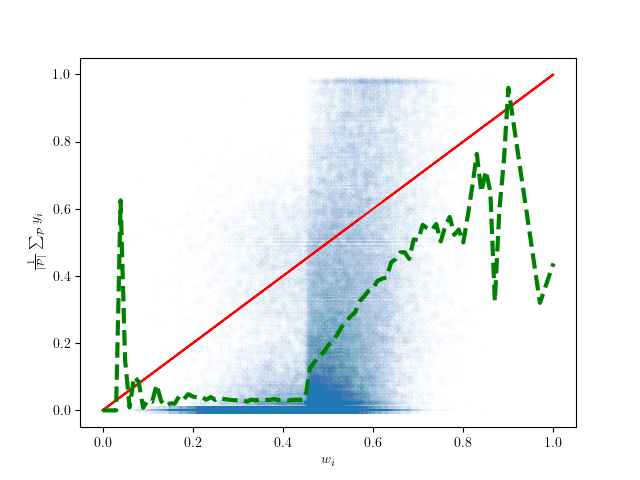
\includegraphics[width=.9\textwidth]{maxcut_n100_p0.15_normal_scatter_weight_prop.png}
	\caption{Scatter plot of proportion $\frac{1}{|\mathcal{P}|} \sum_{\mathcal{P}} y_i$ as a function of the cost $w_i$ of node $i$. Green line is a rolling mean value}

\end{figure}


\end{document}
